\subsection{Версия 1 пайплайна: \texorpdfstring{\(UO_2\)--Zircaloy}{UO2--Zircaloy}}

Эта версия фиксирует штатную пару \(UO_2\)--Zircaloy и использует тепловой ряд GeN-Foam; идентификатор расчета -- \texttt{zircaloy-v1}. Рассматривается один метр твэла с радиусом топлива \(R_f=4.00\,\mathrm{мм}\), зазором \(80\,\mu\mathrm{m}\), оболочкой толщиной \(0.60\,\mathrm{мм}\) и приповерхностным слоем воды толщиной \(\delta_w=100\,\mu\mathrm{m}\) при \(p_w=15.5\,\mathrm{МПа}\). Входной импульс равен \(E_{\mathrm{вв}}=250\,\mathrm{кДж/м}\), а для оболочки используется допустимый предел \(T_{\mathrm{lim},c}=1477\,\mathrm{K}\), а не температура плавления.

Масса воды у оболочки считается из кольцевого контрольного объема:
\[
m_w'=\rho_l \pi\left[(R_c+\delta_w)^2-R_c^2\right].
\]
Для выбранных параметров \(m_w'\approx1.932\,\mathrm{г/м}\). Сначала этот слой испаряется, затем сухой пар может перегреваться. В расчет введено физическое ограничение \(T_s(t)\le T_c(t)\): пар, нагреваемый только через оболочку, не может быть горячее наружной стенки.

\begin{figure}[H]
    \centering
    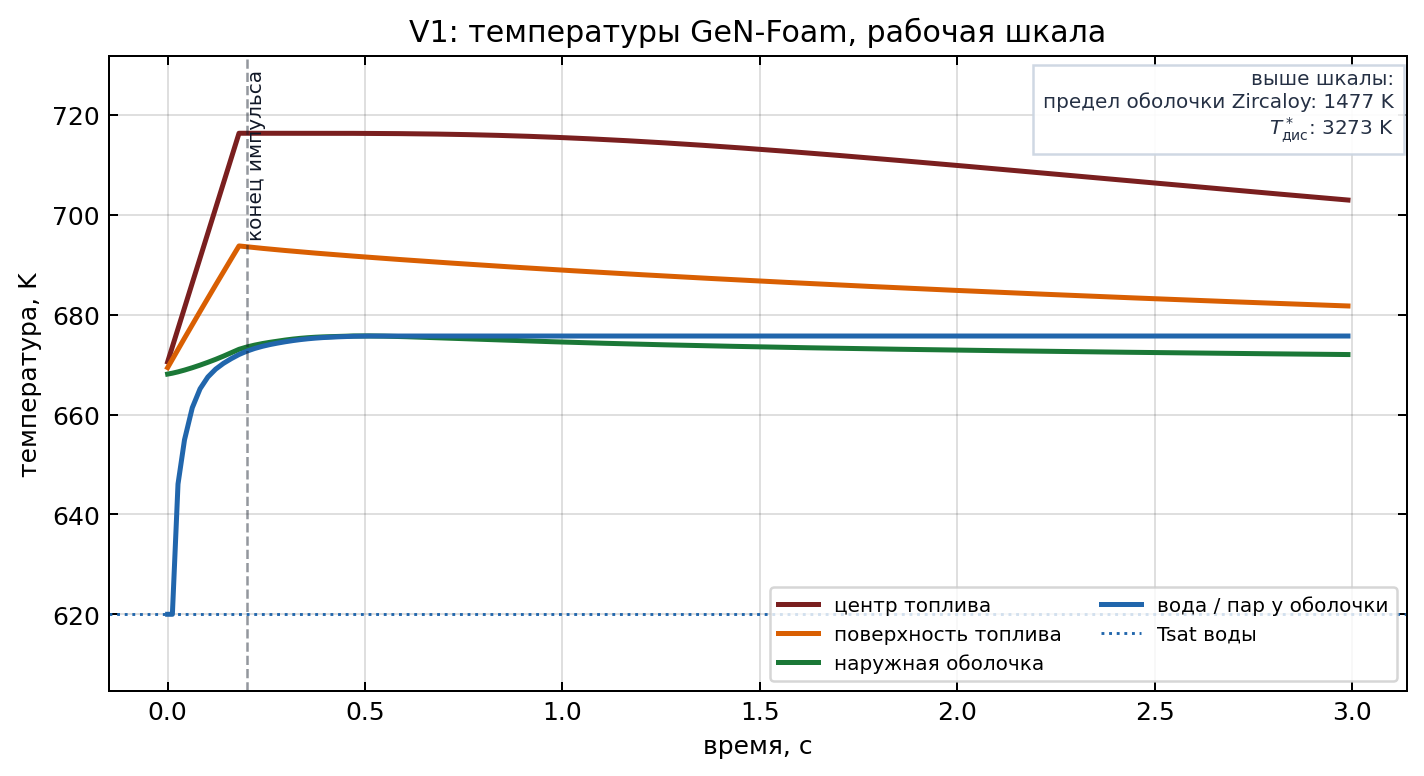
\includegraphics[width=0.82\textwidth]{figures/pipeline_temperature_history.png}
    \caption{Версия 1: история температур \(UO_2\)--Zircaloy при \(E_{\mathrm{вв}}=250\,\mathrm{кДж/м}\). Водно-паровой слой не достигает порога \(T^*_{\mathrm{дис}}=3273\,\mathrm{K}\), а оболочка остается ниже принятого температурного предела.}
    \label{fig:pipelineTemperatureHistory}
\end{figure}

Энергетический график нормирован на полную энергию импульса:
\[
\varepsilon_j(t)=\frac{E_j(t)}{E_{\mathrm{вв}}},
\qquad
j\in\{f,c,s\}.
\]
Здесь \(E_s\) означает энергию в локальном водно-паровом объеме около оболочки после нагрева, испарения и возможного перегрева. В версии 1 водно-паровая область получает \(\varepsilon_s\approx0.962\,\%\) импульса после ограничения температурой стенки. Теплоемкость сухого пара в этом объеме равна \(C_s'\approx5.023\,\mathrm{Дж/(К\cdot м)}\), но до перегрева надо также покрыть скрытую теплоту испарения.

\begin{figure}[H]
    \centering
    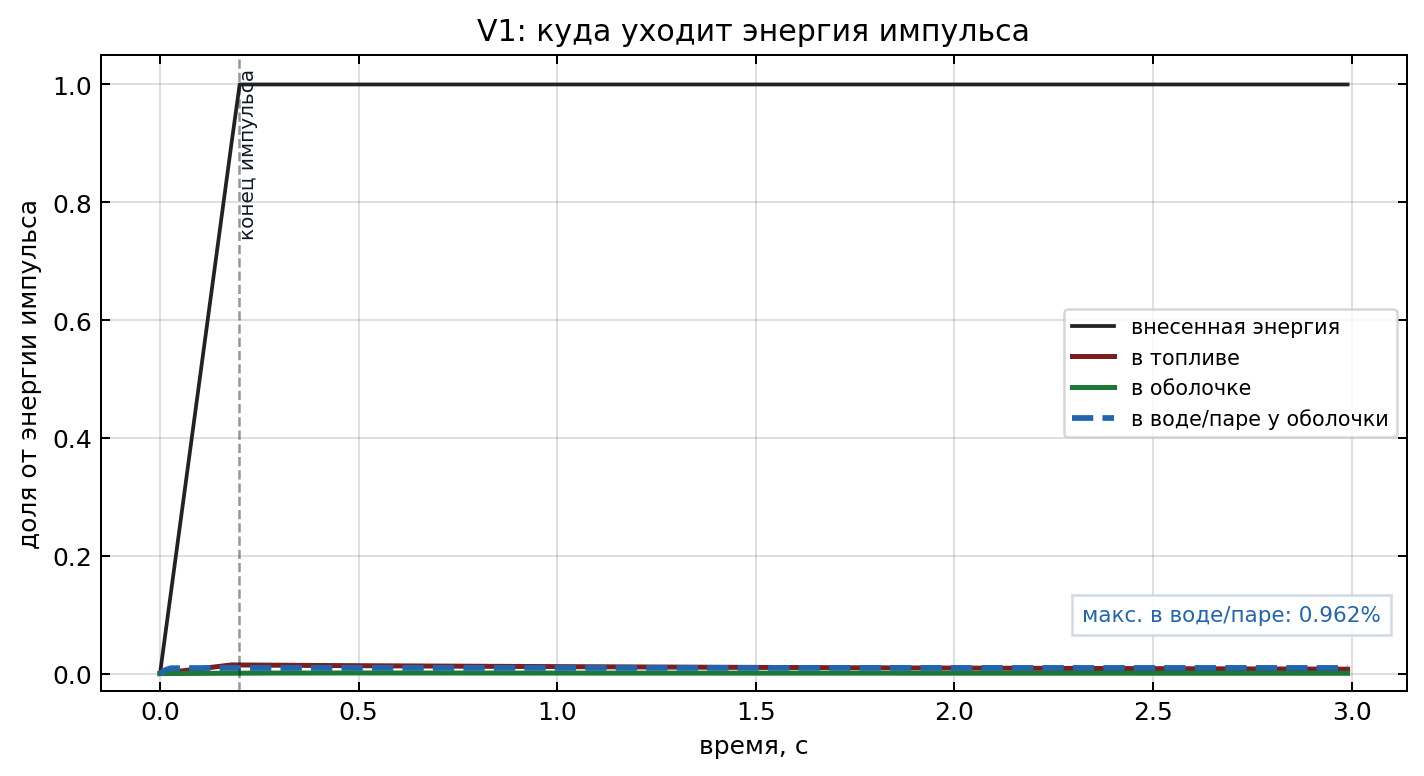
\includegraphics[width=0.82\textwidth]{figures/pipeline_energy_balance.png}
    \caption{Доли энергии импульса, накопленные в топливе, оболочке и водно-паровом слое. Основная часть энергии остается в твердой части твэла или не попадает в локальный водный объем при выбранном ограничении стенкой.}
    \label{fig:pipelineEnergyBalance}
\end{figure}

Малую величину \(\varepsilon_s\) удобно разложить как энергетическую воронку. В строке «топливо и газовый зазор» показана энергия, которая к моменту \(t=3.0\,\mathrm{s}\) еще не дошла до оболочки по выгруженному ряду GeN-Foam. В строке «оболочка» показана энергия, которая уже прошла через зазор, но осталась в металле оболочки и не была передана паровой прослойке.

\begin{table}[H]
    \centering
    \caption{Энергетическая воронка версии 1 к концу расчета. Величины нормированы на \(E_{\mathrm{вв}}=250\,\mathrm{кДж/м}\).}
    \label{tab:pipelineEnergyFunnel}
    \small
    \resizebox{\textwidth}{!}{%
    \begin{tabular}{@{}p{4.2cm}rrrrr@{}}
    \hline
    Звено & Накоплено или не прошло, кДж/м & от \(E_{\mathrm{вв}}\), \% & от входа звена, \% & Прошло дальше, кДж/м & от \(E_{\mathrm{вв}}\), \% \\
    \hline
    Топливо и газовый зазор & 1.86 & 0.744 & 0.744 & 2.53 & 1.01 \\
    Оболочка & 0.13 & 0.052 & 5.10 & 2.40 & 0.962 \\
    \hline
    \end{tabular}
    }
\end{table}

Итоговая энергия в водно-паровом слое составляет \(E_s\approx2.405\,\mathrm{кДж/м}\), или \(0.962\,\%\) от импульса. До последнего расчетного момента с положительным запасом оболочки эта величина составляет \(E_s\approx2.405\,\mathrm{кДж/м}\), или \(0.962\,\%\). Главный ограничитель здесь не полная энергия импульса, а температура наружной оболочки: при \(T_c\ll T^*_{\mathrm{дис}}\) перегретый пар также остается далеко ниже порога диссоциации.

Равновесная химия считается в Cantera по состоянию пара из теплового ряда:
\[
T_s(t),\quad p_s(t),\quad X_0=\{H_2O:1\},
\qquad
m_{H_2}^{eq}=n_{H_2}^{eq}M_{H_2}.
\]
До выхода топлива и оболочки за принятые пределы водно-паровой слой успевает нагреться до \(T_s\approx676\,\mathrm{K}\). Полный расчетный максимум оболочки дает запас \(M_{\mathrm{об}}=T_{\mathrm{lim},c}-T_c^{\max}\approx801\,\mathrm{K}\). Топливо в этой точке еще не является первым ограничением, поскольку \(M_f\approx2404\,\mathrm{K}\).

\begin{table}[H]
    \centering
    \caption{Сводка версии 1: входной импульс и три основных выхода для \(UO_2\)--Zircaloy.}
    \label{tab:pipelineScenarioReport}
    \small
    \resizebox{\textwidth}{!}{%
    \begin{tabular}{@{}p{4.0cm}rp{2.2cm}p{2.4cm}p{2.2cm}p{5.4cm}@{}}
    \hline
    Сценарий & \(E_{\mathrm{вв}}\), кДж/м & \(T_{s,\max}^{M>0}\), K & \(M_{\mathrm{об}}\), K & \(m_{H_2}^{eq}\), г/м & Вывод \\
    \hline
    \(UO_2\)--Zircaloy, версия 1 & 250 & 676 & 801 & \(\ensuremath{7.61\cdot10^{-13}}\) & пределы топлива и оболочки не нарушены, но целевое температурное окно не достигнуто \\
    \hline
    \end{tabular}
    }
\end{table}

Итог версии 1 является отрицательным по термохимическому критерию: в принятом тепловом ряду топливо и оболочка остаются ниже своих пределов, но водно-паровой слой не выходит к выбранному порогу \(T^*_{\mathrm{дис}}\). Для принятого порога \(T^*_{\mathrm{дис}}\) температурный запас пара до нарушения пределов равен \(\Delta T_{\mathrm{зап}}\approx-2597\,\mathrm{K}\), а запас оболочки в полном расчете равен \(M_{\mathrm{об}}\approx801\,\mathrm{K}\).
